\subsection{Performance Results and Analysis}
\label{results}
Of tens of thousands of our sampling runs, we find that the fully populated
cases---i.e. both producer and consumer counts become equal to the total
process count---are most revealing. In particular, we carefully analyze 
the maximum latency of each of the main phases of KAP for these cases 
because this metric represents the critical path of the performance of
many HPC services. For example, distributed 
HPC software would use KVS operations in a coordinated fashion to exchange 
connection information among processes during its bootstrapping 
phase~\cite{LIBI,PMI2}. Unless {\em all} 
of the distributed processes complete their
KVS operations, their communication fabric cannot be established. 

\begin{figure}
  \centering
  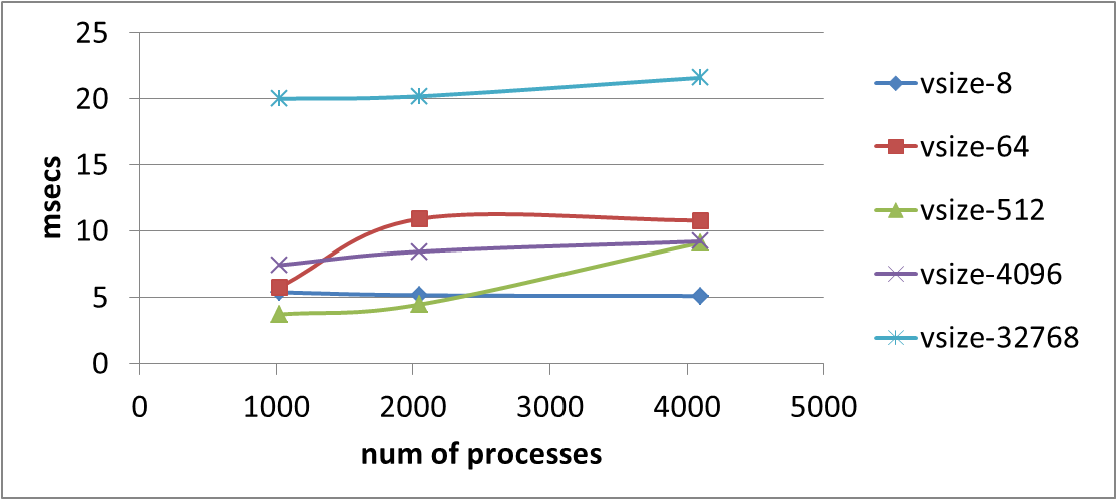
\includegraphics[width=.75\linewidth]{producer}
  \caption{Max latency of producer phase}
  \vspace{-.5cm}	
  \label{fig:prod}
\end{figure}

Figure~\ref{fig:prod} shows the maximum latency of the producer phase
for these cases. Essentially, these plots indicate how well {\tt kvs\_put}
scales as we increase the number of producers. Each plot represents
different value sizes---e.g., vsize-8 refers to value size being
8 bytes. As shown in this graph, the {\tt kvs\_put} simply performs and
scales well. This matches our expectations because objects
are cached in write-back mode at {\tt kvs\_put} time and flushed to the
server at the next consistency event. 

\ifcomments
\marginpar{\tiny DA: I will add data from 8K if I get it on Zin in time.}

\marginpar{\tiny JG: The vsize-32768 requires some explanation}

\begin{figure}[ht]
\centering
\begin{subfigure}[With unique values]{
  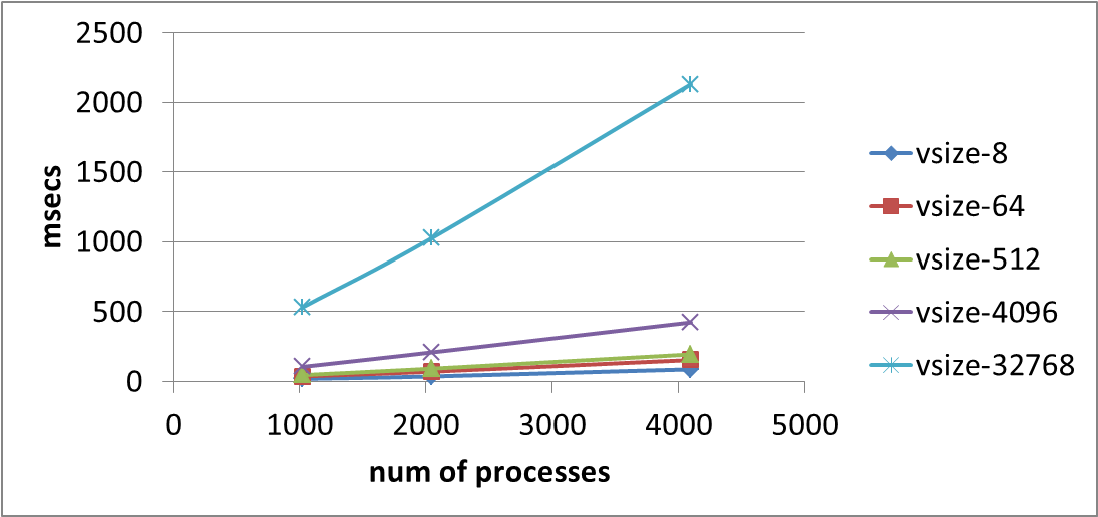
\includegraphics[width=.75\linewidth]{sync}
  \label{fig:sync:noredund}
}%
\end{subfigure}
\begin{subfigure}[With redundant values]{
  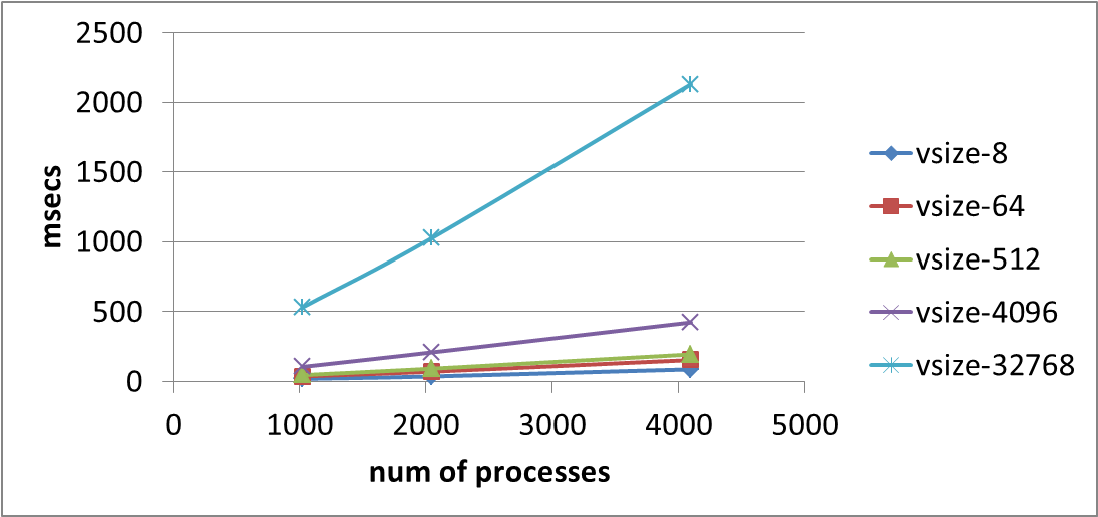
\includegraphics[width=.75\linewidth]{sync}
  \label{fig:sync:redund}
}%
\end{subfigure}
\caption{Max latency of synchronization phase}
\label{fig:sync}
\end{figure}


Moving to the synchronization phase, Fig.~\ref{fig:sync} shows 
how {\tt kvs\_fence} scales during this phase
as we increase the number of producers. 
As with the producer latency,
each plot represents different value sizes.
The most revealing observation is that
fence scalabilty appears to depend on the level of
redundancy in key-value objects that had previously 
been put in. Figure~\ref{fig:sync:redund} 
shows the maximum latency of the synchronization phase
when redundant values are used. It scales
far better than Fig.~\ref{fig:sync:noredund}
where there is zero redundancy in values. 
We theorize that in the former case, fence performs linearly with respect to the number of
producers because these unique values are being {\em concatenated} while
being sent up the tree. It performs logarithmically for the latter case
because redundant values are being {\em reduced} while being sent 
up the tree. %%(MENSION R^2 here?)

\marginpar{\tiny DA: I am speculating a bit for redundant case; my job on cab will confirm or deny this.}

\marginpar{\tiny JG: Dong I can't see any difference between
\ref{fig:sync:redund} and \ref{fig:sync:noredund}.}

\begin{figure}[ht]
\centering
\begin{subfigure}[With single-directory layout]{
  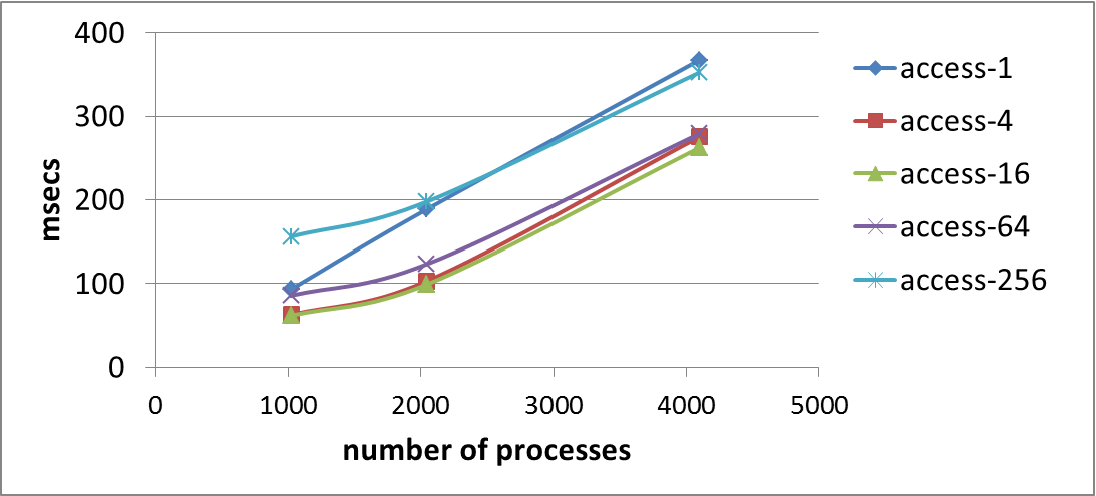
\includegraphics[width=.75\linewidth]{consumer-1-dir}
  \label{fig:cons:dir}
}%
\end{subfigure}
\begin{subfigure}[Improvements with multiple directories]{
  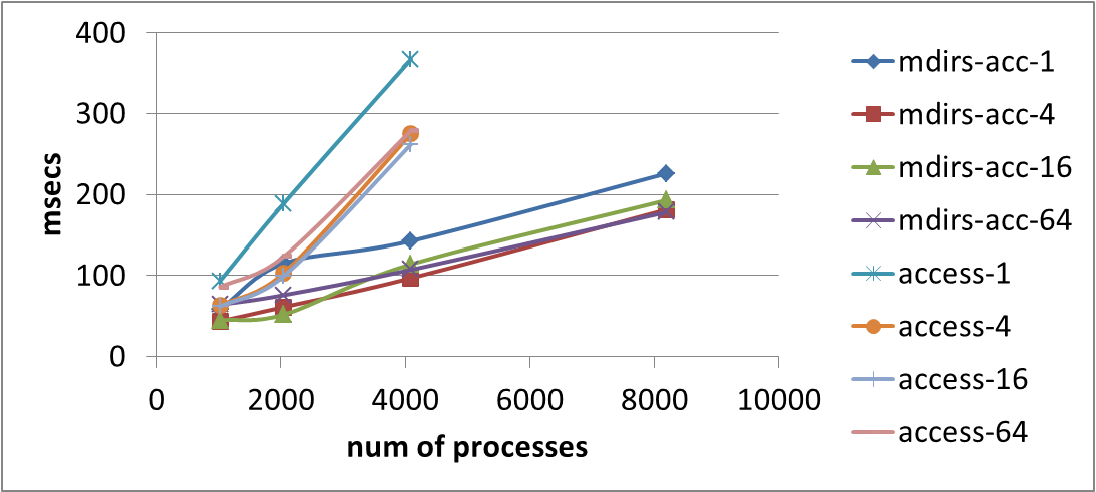
\includegraphics[width=.75\linewidth]{consumer-dist-dir}
  \label{fig:cons:dirs}
}%
\end{subfigure}
\caption{Max latency of consumer phase (value size: 8 bytes)}
\vspace{-.5cm}
\label{fig:consumer}
\end{figure}

Figure~\ref{fig:consumer} shows the maximum latency of the consumer
phase with respect to various parameter settings. 
These results suggest how well {\tt kvs\_get}
scales, as we increase the number of consumers. Each plot represents
the latency when each consumer reads different numbers of 
objects, e.g., the access-4 plot represents each consumer reading
4 distinct objects.  While these figures show only the performance of reading
objects 8 bytes in size, we observe that the general 
scalability trends are similar at different value sizes.
Suprisingly, we see little change in performance when value sizes
exceed the 42-byte store-by-reference limit.

Figure~\ref{fig:cons:dir} shows the maximum latency of {\tt kvs\_get}
when the target key-value objects are all stored in a single
KVS directory. The latency is quite high and also increases
linearly, as we increase the number of consumers. 
It appears that the poor performance and scaling behavior 
are attributed to KVS replication granularity and 
the fact that the objects are stored in a single directory.

When {\tt kvs\_get} cannot be satisfied by the local KVS replica,
our system ensures that the entire directory where
the requested object resides is replicated on
all of the ancestor CMB daemons that are along the direct path 
to the root. With our access pattern where all objects
are read collectively by consumers, this means the latency is 
$log_2(C) \times T_{replicate}(G)$, where C is the consumer count, and G is the 
total amount of data in the master KVS server.
Thus, the max latency increase for every doubling of consumers is 
$\frac{log_2(2C) \times T_{replicate}(2G)}{log_2(C) \times T_{replicate}(G)}$.
Generally, this would approach 2, 
as we continue to increase the number of consumers,
and our data match with this model.

We can improve this behavior by storing objects across multiple
directories. With such an organization, the size of replicas 
would decrease as we go down the CMB tree. This is of course only when
each consumer reads only a small fraction of data. In another
word, if each consumer read all of the data in KVS, the latency
would be same as the single directory case. 
Figure~\ref{fig:cons:dir} shows the improvements 
when we spread objects into multiple directories by
keeping the number of objects per directory constant: 128.
Label {\tt mdir-acc-k} refers to the same access pattern as {\tt access-k} 
except the accessing objects are stored across multiple directories.


For the case where the size of replicas 
decreases as a function of tree levels, 
we can model the latency as a geometric series. For example, at tree height being $h$,
the latency would be 
$T_{replicate}(G) + T_{replicate}(\frac{G}{2}) + T_{replicate}(\frac{G}{4}) + ... + T_{replicate}(\frac{G}{2^h})$, 
where each term represents the latency of replication per level.
This would approach $2T_{replicate}(G)$. Thus, its improvement over the single
directory scheme is: $\frac{log_2(C) \times T_{replicate}(G)}{2 T_{replicate}(G)}$.
Roughly speaking, the improvements would be on the order of 
$\frac{1}{2}log_2(C)$. The improvements would be linearly 
greater as we increase the scale and our measurements agree with this. 

While significant, we note that a smarter KVS data layout scheme alone
can still fall short of reaching extreme scale. Our model tells us that the latency
will grow linearly when $G$ grows with the scale. 
Say, $G$ doubles every time you double the number of consumers, our geometric series
model predicts the latency will also double:
$\frac{2T_{replicate}(2G)}{2T_{replicate(G)}}$ becomes 
on the order of 2. With the current scheme, the only true way to gain logarithmic
scaling is when $G$ stays constant regardless of scale. 
In a later section, we will discuss some of our plans 
to exploit the understanding we gain from the evaluation. 


